\section{(E)PTAS for FVS-BCL Problem Using Baker's Technique}

\noindent In this section we provide the necessary definitions, lemmas and theorems to demonstrate how to obtain an EPTAS for the problem 
we defined in \ref{FVS-BCL}, namely FVS-BCL. In the preliminaries we gave two examples of how to construct algorithms using Baker's technique 
and how to further analyse them. In the same fashion we now construct Algorithm \ref{alg:ufvsbcl} and reason for its effectiveness.

\noindent In the following algorithm we use the letter $\ell$ for the outerplanarity of each subgraph, i.e. each $G_{i, j}$ that we 
define on line 4 in Algorithm~\ref{alg:ufvsbcl} is $\ell$-outerplanar.

\begin{algorithm}[H]
    \caption{Baker's technique for the unweighted FVS-BCL}
    \label{alg:ufvsbcl}
    \begin{algorithmic}[1]
    \REQUIRE Planar graph $G = (V, E)$, parameter $\ell$
    \ENSURE $(1 + \epsilon)$-approximation for \textsc{FVS-BCL}
    \STATE Perform \textsc{BFS} from some arbitrary vertex $r$
    \STATE $S \leftarrow \emptyset$

    $i$: \textit{shift}; $j$: \textit{slice}

    \FOR{each $i = 0$ to $\ell-1$}
        \STATE Let $G_{i, j}$ be the subgraph induced on vertices at levels $j \times k + i$ through $(j+1) \times k + i$ for $0 \leq i < k$.
        \STATE $\forall j \text{ compute }  S_{i, j}$, the min. \textsc{VC} of $G_{i, j}$.
        \STATE $\forall j \text{ let } S_i = \bigcup_{j} S_{i, j}$
        \STATE $S \leftarrow S \cup S_i$
    \ENDFOR
    \RETURN $S_{i*}$ from $S$ with minimum cardinality
    \end{algorithmic}
\end{algorithm}

\noindent In the analysis of the algorithm we are going to need three lemmas in order 
to prove that Algorithm~\ref{alg:ufvsbcl} obtains a $(1 + 2/\ell)$-approximation of the 
optimum solution.

\refstepcounter{definition}
\begin{mydefinition}[Optimum solution bound]{Lemma}
    \label{lemma-one}

    Let $S_{i, j}$ be an optimum solution for $G_{i, j}$ for some shift $i$ and slice $j$, 
    let $F \equiv OPT$ be the optimum solution in $G$ and let $F_{i, j} = G_{i, j} \cap F$. 
    In the unweighted case we claim that: \[|S_{i, j}| \leq |F_{i, j}|\text{.}\]

    We will say that $F_{i, j}$ is a FVS-BCL of $G_{i, j}$, not necessarily the one of minimum cardinality.

\end{mydefinition}

\noindent For now we do not argue about how we obtain an optimum solution, in further sections we will show how 
to to get it using tree decompositions and dynamic programming, but for now we argue that this inequality 
holds in each subgraph $G_{i, j}$.

\noindent We first argue that in each subgraph $G_{i, j}$, the set $F_{i, j}$ contains a vertex that 
breaks every 4-cycle.  Let us fix a slice and shift $a$ and $b$ and take a look at the subgraph $G_{a, b}$, 
the optimal solution for it $S_{a, b}$ and the set $F_{a, b}$. Notice that, much like in the Vertex Cover
analysis, no vertex in $V(G) \backslash V(G_{a, b})$ can break any 4-cycle that is contained within 
$G_{a, b}$. Therefore $F_{a, b}$ must contain a vertex that hits every 4-cycle or it will not be 
a solution in $G_{a, b}$ and subsequently in $G$. From this and the fact that $S_{a, b}$ is an optimum 
solution for $G_{a, b}$ we conclude that: \[|S_{a, b}| \leq |F_{a, b}|\text{.}\]
for some $(a, b)$, therefore it holds $\forall (i, j)$. 

\noindent One must confront the fact that notation is abused throughout the paper, especially when it 
comes down to $j$, the slice variable. When we say that a statement holds for all values $i$ and
$j$, we mean that it holds for the subgraphs that these variables outline. We will sketch an example 
to deepen our understanding of Lemma~\ref{lemma-one}. Moreover, we are going to explore one avenue 
that gives rise to an inequality in the lemma.



\begin{center}
    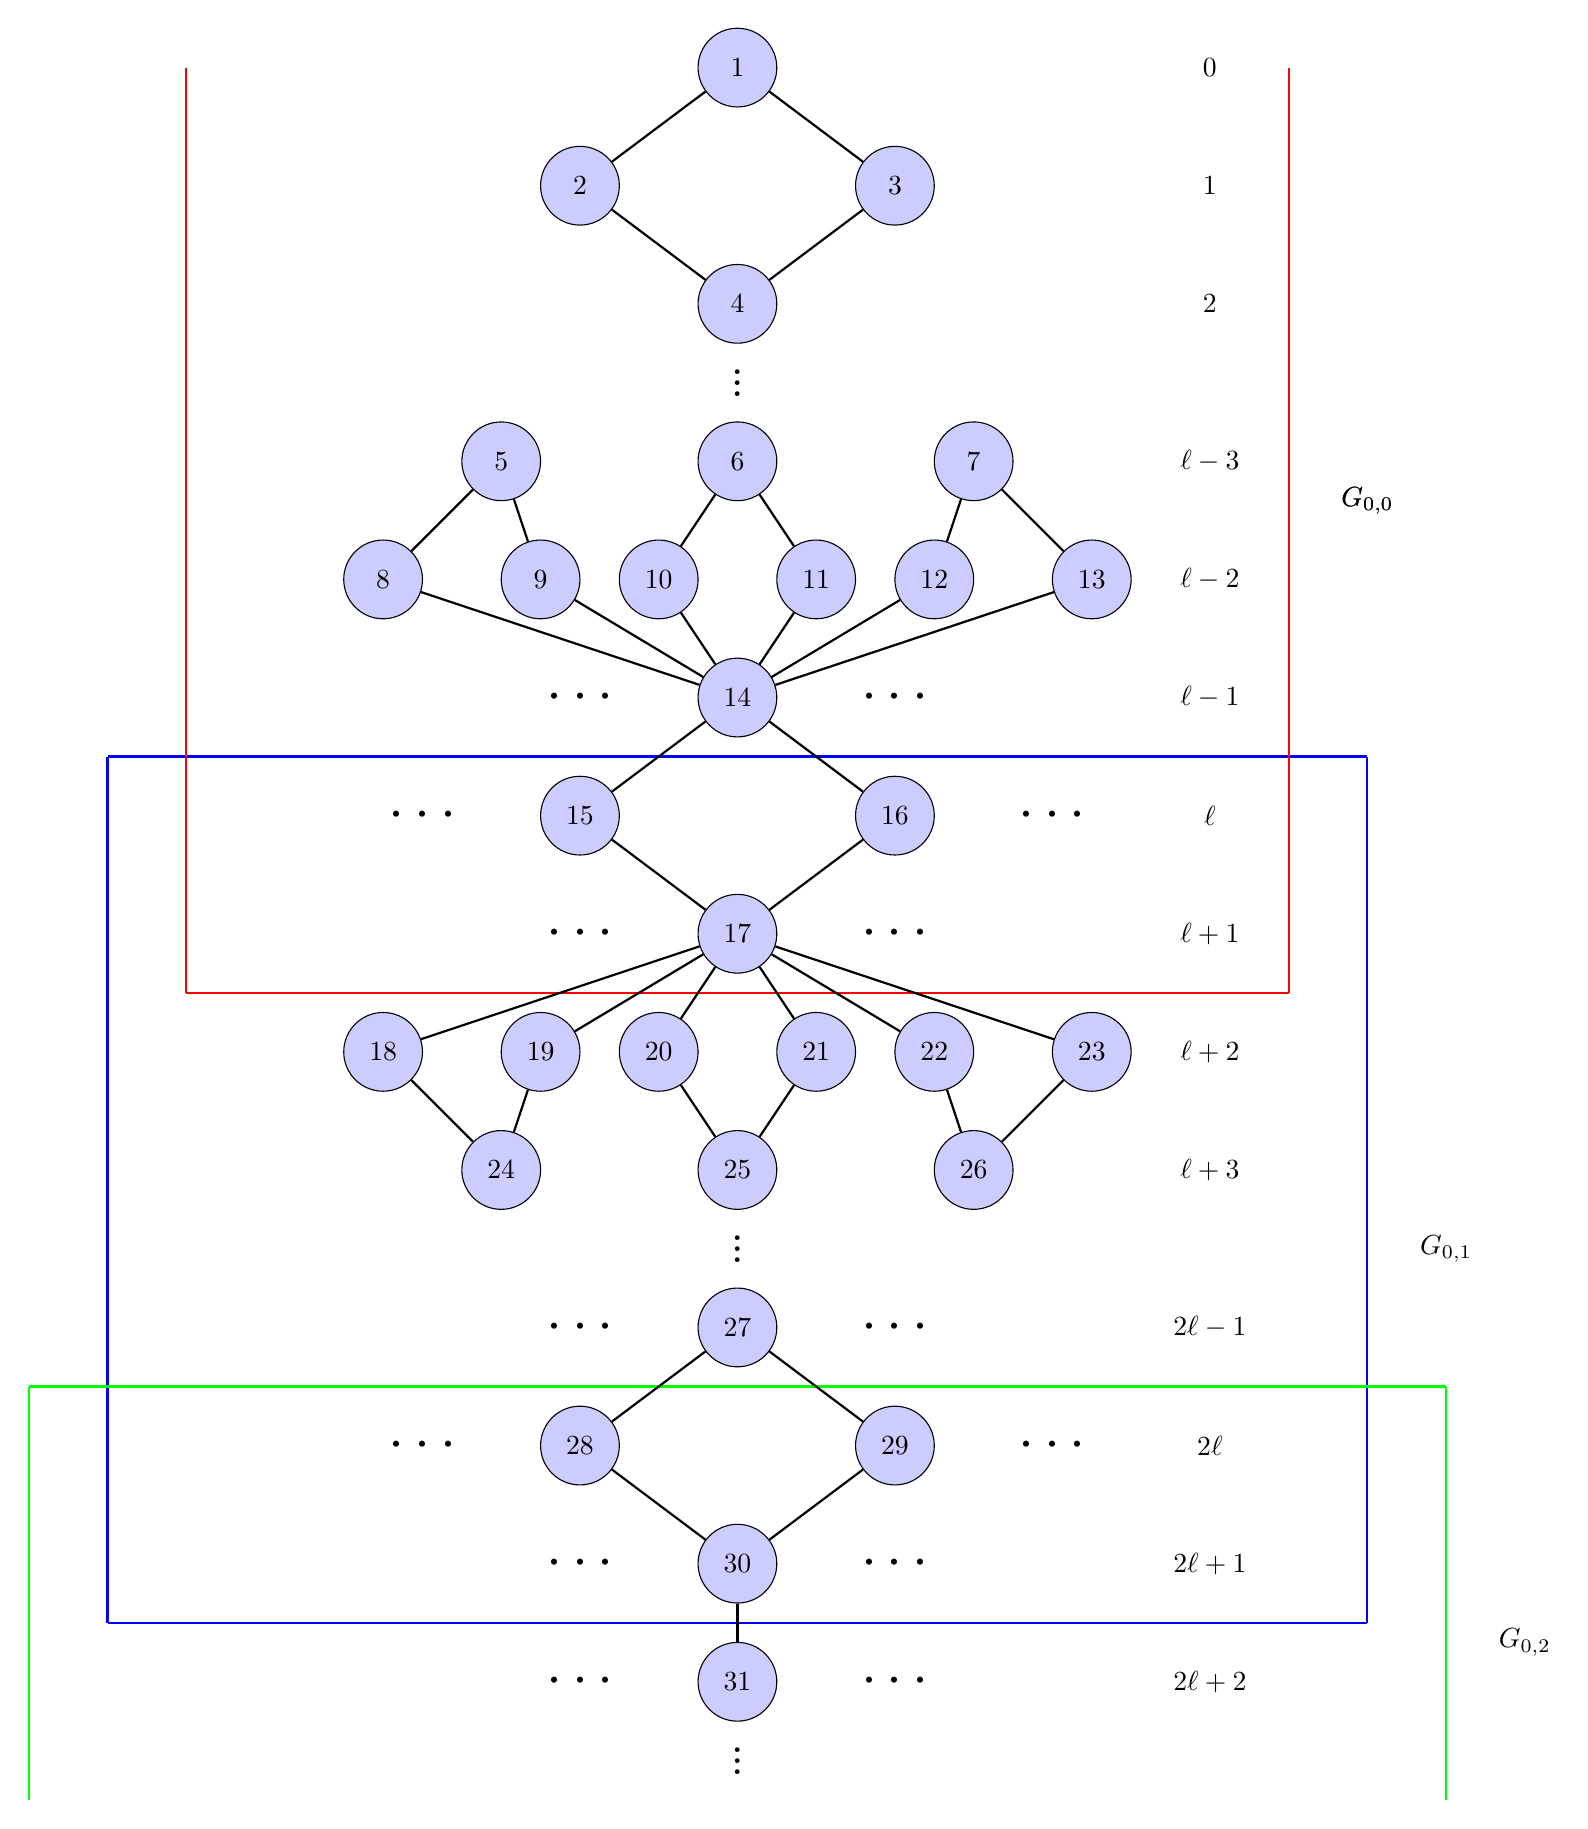
\begin{tikzpicture}
        % Level 0 (Root node)
        \node[circle, draw, fill=blue!20, minimum size=10mm] (1) at (0, 0) {1};

        % Level 1
        \node[circle, draw, fill=blue!20, minimum size=10mm] (2) at (-2, -1.5) {2};
        \node[circle, draw, fill=blue!20, minimum size=10mm] (3) at (2, -1.5) {3};

        % Level 2
        \node[circle, draw, fill=blue!20, minimum size=10mm] (4) at (0, -3) {4};

        % Dotted vertical line indicating further levels
        \node[draw=none] at (0, -3.9) { \huge $\vdots$ };

        % Level l-3
        \node[circle, draw, fill=blue!20, minimum size=10mm] (5) at (-3, -5){5};
        \node[circle, draw, fill=blue!20, minimum size=10mm] (6) at (0, -5) {6};
        \node[circle, draw, fill=blue!20, minimum size=10mm] (7) at (3, -5) {7};

        % Level l-2
        \node[circle, draw, fill=blue!20, minimum size=10mm] (8) at (-4.5, -6.5){8};
        \node[circle, draw, fill=blue!20, minimum size=10mm] (9) at (-2.5, -6.5) {9};
        \node[circle, draw, fill=blue!20, minimum size=10mm] (10) at (-1, -6.5) {10};
        \node[circle, draw, fill=blue!20, minimum size=10mm] (11) at (1, -6.5) {11};
        \node[circle, draw, fill=blue!20, minimum size=10mm] (12) at (2.5, -6.5) {12};
        \node[circle, draw, fill=blue!20, minimum size=10mm] (13) at (4.5, -6.5) {13};
        
        % Level l-1
        \node[circle, draw, fill=blue!20, minimum size=10mm] (14) at (0, -8){14};

        \node[draw=none] at (2, -8) {\huge $\cdots$};
        \node[draw=none] at (-2, -8) {\huge $\cdots$};

        % Vertical line between levels l-1 and l
        \draw[thick, blue] (-8, -8.75) -- (8, -8.75);
        \draw[thick, blue] (-8, -8.75) -- (-8, -19.75);
        \draw[thick, blue] (8, -8.75) -- (8, -19.75);
        \draw[thick, blue] (-8, -19.75) -- (8, -19.75);
        \node[draw=none] at (9, -15) {$G_{0, 1}$};

        % Level l
        \node[circle, draw, fill=blue!20, minimum size=10mm] (15) at (-2, -9.5){15};
        \node[circle, draw, fill=blue!20, minimum size=10mm] (16) at (2, -9.5){16};

        \node[draw=none] at (4, -9.5) {\huge $\cdots$};
        \node[draw=none] at (-4, -9.5) {\huge $\cdots$};

        % Level l+1
        \node[circle, draw, fill=blue!20, minimum size=10mm] (17) at (0, -11){17};
        
        % Vertical line between levels l+1 and l+2
        \draw[thick, red] (-7, -11.75) -- (7, -11.75);
        \draw[thick, red] (-7, -11.75) -- (-7, 0);
        \draw[thick, red] (7, -11.75) -- (7, 0);
        \node[draw=none] at (8, -5.5) {$G_{0, 0}$};

        % Horizontal dots on level l+1
        \node[draw=none] at (2, -11) {\huge $\cdots$};
        \node[draw=none] at (-2, -11) {\huge $\cdots$};

        % Level l+2
        \node[circle, draw, fill=blue!20, minimum size=10mm] (18) at (-4.5, -12.5){18};
        \node[circle, draw, fill=blue!20, minimum size=10mm] (19) at (-2.5, -12.5) {19};
        \node[circle, draw, fill=blue!20, minimum size=10mm] (20) at (-1, -12.5) {20};
        \node[circle, draw, fill=blue!20, minimum size=10mm] (21) at (1, -12.5) {21};
        \node[circle, draw, fill=blue!20, minimum size=10mm] (22) at (2.5, -12.5) {22};
        \node[circle, draw, fill=blue!20, minimum size=10mm] (23) at (4.5, -12.5) {23};
        
        % Level l+3
        \node[circle, draw, fill=blue!20, minimum size=10mm] (24) at (-3, -14){24};
        \node[circle, draw, fill=blue!20, minimum size=10mm] (25) at (0, -14) {25};
        \node[circle, draw, fill=blue!20, minimum size=10mm] (26) at (3, -14) {26};

        % Dotted vertical line indicating further levels
        \node[draw=none] at (0, -14.9) { \huge $\vdots$ };

        % Level 2l - 1
        \node[circle, draw, fill=blue!20, minimum size=10mm] (27) at (0, -16) {27};

        \node[draw=none] at (2, -16) {\huge $\cdots$};
        \node[draw=none] at (-2, -16) {\huge $\cdots$};

        % Vertical line between levels l+1 and l+2
        \draw[thick, green] (-9, -16.75) -- (9, -16.75);
        \draw[thick, green] (-9, -16.75) -- (-9, -22);
        \draw[thick, green] (9, -16.75) -- (9, -22);
        \node[draw=none] at (8, -5.5) {$G_{0, 0}$};

        % Level 2l
        \node[circle, draw, fill=blue!20, minimum size=10mm] (28) at (-2, -17.5) {28};
        \node[circle, draw, fill=blue!20, minimum size=10mm] (29) at (2, -17.5) {29};
        
        \node[draw=none] at (4, -17.5) {\huge $\cdots$};
        \node[draw=none] at (-4, -17.5) {\huge $\cdots$};

        % Level 2l+1
        \node[circle, draw, fill=blue!20, minimum size=10mm] (30) at (0, -19) {30};

        \node[draw=none] at (2, -19) {\huge $\cdots$};
        \node[draw=none] at (-2, -19) {\huge $\cdots$};

        % Level 2l+2
        \node[circle, draw, fill=blue!20, minimum size=10mm] (31) at (0, -20.5) {31};

        \node[draw=none] at (2, -20.5) {\huge $\cdots$};
        \node[draw=none] at (-2, -20.5) {\huge $\cdots$};

        % Dotted vertical line indicating further levels
        \node[draw=none] at (0, -21.4) { \huge $\vdots$ };

        \node[draw=none] at (10, -20) {$G_{0, 2}$};


        % Draw edges for BFS with renumbered vertices
        \foreach \I/\j in {1/2, 1/3, 2/4, 3/4, 5/8, 5/9, 8/14, 9/14, 6/10, 6/11, 10/14, 11/14,
        7/12, 7/13, 12/14, 13/14, 14/15, 14/16, 15/17, 16/17, 17/18, 17/19, 17/20, 17/21, 17/22, 17/23,
        18/24, 19/24, 20/25, 21/25, 22/26, 23/26, 27/28, 27/29, 28/30, 29/30, 30/31}
            \draw[thick] (\I) -- (\j);

        \node[draw=none] at (6, 0) {0};
        \node[draw=none] at (6, -1.5) {1};
        \node[draw=none] at (6, -3) {2};

        \node[draw=none] at (6, -5) {$\ell-3$};
        \node[draw=none] at (6, -6.5) {$\ell-2$};
        \node[draw=none] at (6, -8) {$\ell-1$};
        \node[draw=none] at (6, -9.5) {$\ell$};
        \node[draw=none] at (6, -11) {$\ell+1$};
        \node[draw=none] at (6, -12.5) {$\ell+2$};
        \node[draw=none] at (6, -14) {$\ell+3$};

        \node[draw=none] at (6, -16) {$2\ell-1$};
        \node[draw=none] at (6, -17.5) {$2\ell$};
        \node[draw=none] at (6, -19) {$2\ell+1$};

        \node[draw=none] at (6, -20.5) {$2\ell+2$};

    \end{tikzpicture}
\end{center}

\noindent Let $G$ look like the graph we sketched on the previous page. The vertical dots help us 
clarify the levels while the horizontal signify that there may be other vertices of interest. However, 
there are vertices we would like to inspect, specifically vertices with labels $14$ and $17$. Let 
$v_{14}, v_{17} \in F$. What follows is that $v_{14}, v_{17} \in F_{0, 0}$. The cycles that give us
reason to claim that $v_{14} \in F$ are all within $G_{0, 0}$. Therefore, it holds that
Algorithm~\ref{alg:ufvsbcl} will have $v_{14} \in S_{0, 0}$. However, the same does not hold for 
$v_{17}$, the cycles that it is a part of are in $G_{0, 1}$ and thus $v_{17} \notin S_{0, 0}$, while 
$v_{17} \in F_{0, 0}$. Thus we will be counting $v_{17}$ twice when we are combining the solutions
$F_{i, j}$, once in $F_{0, 0}$ and once in $F_{0, 1}$. This is what enables us to obtain an upper bound 
for $S$.